\documentclass[a4paper,11pt]{article}

\usepackage{amsmath}
\usepackage{amssymb}
\usepackage{amsthm}
\usepackage{graphicx}
\usepackage{enumerate}
\usepackage{stmaryrd}
\usepackage{setspace}
\usepackage{tikz}
\usepackage{cleveref}
\usetikzlibrary{matrix}
%you can add more packages using the same code above

%------------------

%\setlength{\topmargin}{0.0in}
%\setlength{\textheight}{10in}
%\setlength{\oddsidemargin}{0.0in}
%\setlength{\evensidemargin}{0.0in}
%\setlength{\textwidth}{6.5in}

%-------------------
\newtheorem{theorem}{Theorem}[section]
\newtheorem{proposition}[theorem]{Proposition}
\newtheorem{lemma}[theorem]{Lemma}
\newtheorem{corollary}[theorem]{Corollary}
\newtheorem{conjecture}[theorem]{Conjecture}


\theoremstyle{definition}
\newtheorem{definition}[theorem]{Definition}
\newtheorem*{example}{Example}

%------------------

%Everything before begin document is called the pre-amble and sets out how the document will look
%It is recommended you don't touch the pre-amble until you are familiar with LateX

\begin{document}

\title{Crash-Deterministic Property in Agda}
%\author{Lin Tzu Chi}
%\date{}
\maketitle

\begin{abstract}
	We have proved crash-deterministic properties in Agda.
\end{abstract}

%The following code is not run because of the percentage sign, but you might find it useful for future work
% \tableofcontents

\section{Datatypes}

To define the theorem, following datatypes(definitions) are required:

\begin{align*}
%\noalign{\center{\small{State of Spec, a pair of two mappings from Address to Data, representing abstracted volatile and stable states respectively.}}}
	\mathit{Addr}, \mathit{Data} &: \mathit{undefined}\\
	\mathit{State} &: (Addr \to Data) \times (Addr \to Data)\\
%\noalign{\center{\small{State of Prog, we don't have to know the details.}}}
	\mathit{RawState^P} &: \mathit{undefined}\\
	\mathit{State^P} &: \{ \mathit{rs} \in \mathit{RawState^P} | \mathit{RI(rs) \lor CI(rs)} \}\\
	\mathit{Action} &: \{w(Addr, Data), f, r, w^c, f^c, r^c\}\\
	\mathit{Fragment} &: [\mathit{Action}]\\
\end{align*}

$\mathit{State}$ is the type of states in the operational specification, which is a pair of mappings from $Addr$ to $Data$, the types of which are both $\mathit{undefined}$. these two mappings represent the volatile and stable memory state of the specification.  By $\mathit{undefined}$ we mean that since the actual meanings of some types are proof irrelevant, they are abstracted as module parameters in Agda, and can be given concrete meanings if needed in further works.

For states in the actual program, the meaning of $\mathit{RawState^P}$ is also proof irrelevant. $\mathit{State^P}$ is the type of states in the program we care \---- states that satisfies Representation Invariance or Crash Invariance. $\mathit{Fragment}$ is a list of $\mathit{Action}$.

And we need functions to represent actions of reading from states:
\begin{align*}
	read &: \mathit{RawState^P} \to (\mathit{Addr} \to \mathit{Data})\\
	volatile &: \mathit{State} \to (\mathit{Addr} \to \mathit{Data})\\
	stable &: \mathit{State} \to (\mathit{Addr} \to \mathit{Data})
\end{align*}

\newpage

Single-step transitions are defined as relations on two states indexed by $\mathit{Action}$, and multi-step transitions as their reflextive transitive clousures (indexed by $\mathit{Fragmant}$):
\begin{align*}
	\llbracket \mathit{Action} \rrbracket, \llbracket \mathit{Fragment} \rrbracket^* &: \text{Relation on $\mathit{State \times State}$.}\\
	\llbracket \mathit{Action} \rrbracket^R, \llbracket \mathit{Fragment} \rrbracket^{R*} &: \text{Relation on $\mathit{RawState^P \times RawState^P}$.}\\
	\llbracket \mathit{Action} \rrbracket^P, \llbracket \mathit{Fragment} \rrbracket^{P*} &: \text{Relation on $\mathit{State^P \times State^P}$.}\\
\end{align*}

In other words, states $s$, $s'$ satisfies $s \llbracket \mathit{ac} \rrbracket^P s'$ implies $\mathit{RI(s)}$(when $\mathit{ac} \in \{w, f, w^c, f^c\}$) or $\mathit{CI(s)}$(when $\mathit{ac} \in \{r, r^c\}$).

For any two states $s$, $s'$ in specification, $s \llbracket \mathit{Action} \rrbracket s'$ if and only if for each $\mathit{Action}$, followings hold:
\begin{align*}
	s \llbracket w(addr, data) \rrbracket s' &: \mathit{volatile(s)[addr \mapsto data]} \doteq \mathit{volatile(s')}\\
	& \ \  \land stable(s) \doteq stable(s')\\
	s \llbracket f \rrbracket s' &: \mathit{volatile(s)} \doteq \mathit{volatile(s')} \land \mathit{volatile(s)} \doteq \mathit{stable(s')}\\
	s \llbracket r \rrbracket s' &: \mathit{stable(s)} \doteq \mathit{volatile(s')} \land \mathit{stable(s)} \doteq \mathit{stable(s')}\\
	s \llbracket w^c \rrbracket s' &: \mathit{stable(s)} \doteq \mathit{stable(s')}\\
	s \llbracket f^c \rrbracket s' &: \mathit{volatile(s)} \doteq \mathit{stable(s')} \lor \mathit{stable(s)} \doteq \mathit{stable(s')}\\
	s \llbracket r^c \rrbracket s' &: \mathit{stable(s)} \doteq \mathit{stable(s')}
\end{align*}

Important predicates are defined as follows:
\begin{align*}
	\mathit{Init^P(rs : RawState^P)} &: \text{$\mathit{rs}$ is an initial state.}\\
	\mathit{RI(rs : RawState^P)} &: \text{$\mathit{rs}$ satisfies Representation Invariance.} \\
	\mathit{CI(rs : RawState^P)} &: \text{$\mathit{rs}$ satisfies Crash Invariance.} \\
	\mathit{AR(rs : RawState^P, s : State)} &: \text{$\mathit{rs}$ and $s$ satisfies Abstract Relation.} \\
	\mathit{CR(rs : RawState^P, s : State)} &: \text{$\mathit{rs}$ and $s$ satisfies Crash Relation.} \\
\end{align*}

Every one of which has its type $\mathit{undefined}$, with reason stated above. 

Lemmas that are trivial or have been proved with theorem prover can be assumed here:
\begin{align*}
	\mathit{ExistsSpec} &: \forall t \in \mathit{State}, a \in \mathit{Action} \ldotp \exists t' \in \mathit{State} \ldotp t \llbracket a \rrbracket t'\\
	\mathit{Observational Equivalence} &: \forall \mathit{rs} \in \mathit{RawState^P},s \in \mathit{State} \ldotp\\
	 & \quad \mathit{RI(rs)} \land \mathit{AR(rs, s)} \implies \mathit{read(rs)} \doteq \mathit{volatile(t)}\\
	\mathit{initialisation} &: \forall \mathit{rs} \in \mathit{State^P} \ldotp\\
	 &\quad \mathit{Init(rs) \implies \exists s \in State \ldotp RI(rs) \land AR(rs, s)}\\
	\mathit{PerOperationCorrectness} &:\\
	 \mathit{StateInvariance} &: \forall s, s' \in \mathit{State^P},\\
	...	 &\quad \mathit{ac} \in \{w, f\} \ldotp \mathit{s \llbracket ac \rrbracket^P s' \implies RI(s')}\\
	...	 &\quad \mathit{ac} \in \{w^c, f^c\} \ldotp \mathit{s \llbracket ac \rrbracket^P s' \implies CI(s')}\\
	...	 &\quad \mathit{ac} \in \{r\} \ldotp \mathit{s \llbracket ac \rrbracket^P s' \implies RI(s')}\\
	...	 &\quad \mathit{ac} \in \{r^c\} \ldotp \mathit{s \llbracket ac \rrbracket^P s' \implies CI(s')}\\
	RelationInvariance &: \mathit{\forall s, s' \in State^P, t, t' \in State,}\\
	...	& \quad \mathit{ac} \in \{w, f\} \ldotp \mathit{s \llbracket ac \rrbracket^P s' \land t \llbracket ac \rrbracket t' \land AR(s, t) \implies AR(s', t')}\\
	...	& \quad \mathit{ac} \in \{w^c, f^c\} \ldotp \mathit{s \llbracket ac \rrbracket^P s' \land t \llbracket ac \rrbracket t' \land AR(s, t) \implies CR(s', t')}\\
	...	& \quad \mathit{ac} \in \{r\} \ldotp \mathit{s \llbracket ac \rrbracket^P s' \land t \llbracket ac \rrbracket t' \land CR(s, t) \implies AR(s', t')}\\
	...	& \quad \mathit{ac} \in \{r^c\} \ldotp \mathit{s \llbracket ac \rrbracket^P s' \land t \llbracket ac \rrbracket t' \land CR(s, t) \implies CR(s', t')}\\
\end{align*}

We can now proceed to define the lemmas.

\subsection{Lemmas}

\begin{lemma}\label{lemma-2-1}
\begin{align*}
	\forall s, s', s'' \in \mathit{State} \ldotp s \llbracket \mathit{(w \lor f)\ast} \cdot f \rrbracket^* s' \land s' \llbracket \mathit{w\ast} \cdot w^c \cdot \mathit{r^c\ast} \cdot r \rrbracket^* s'' \\
	  \implies \mathit{volatile(s')} \doteq \mathit{volatile(s'')}
\end{align*}
\end{lemma}
\begin{proof}
	$s'$ is related from some $s \in \mathit{State}$ by $\llbracket f \rrbracket$, so
		$$\mathit{volatile(s')} \doteq \mathit{volatile(s)} \doteq \mathit{stable(s')}$$
	since any state related by $\llbracket w \rrbracket$, $\llbracket w^c \rrbracket$ or $\llbracket r^c \rrbracket$ has it's stable unchanged from the state it's related from, there's an intermidiate state $s'_i$ such that
		$$s' \llbracket {w*} \cdot w^c \cdot {r^c *} \rrbracket^* s'_i \land s'_i \llbracket r \rrbracket s'' \land stable(s') \doteq stable(s'_i)$$
	finally, by $\llbracket r \rrbracket$ we know that $\mathit{stable(s'_i) \doteq volatile(s'')}$, thus we have
		$$\mathit{volatile(s') \doteq stable(s') \doteq stable(s'_i) \doteq volatile(s'')}$$
\end{proof}

\begin{lemma}\label{lemma-2-2}
\begin{multline*}
      \forall s, s', s'', s''' \in \mathit{State} \ldotp \\
      s \llbracket \mathit{(w \lor f)\ast} \cdot f \rrbracket s' \land
	  s' \llbracket \mathit{w\ast} \rrbracket^{P*} s'' \land
	  s'' \llbracket f^c \cdot \mathit{r^c\ast} \cdot r \rrbracket^{P*} s'''\\ \implies \mathit{volatile(s')} \doteq \mathit{volatile(s''')} \lor \mathit{volatile(s'')} \doteq \mathit{volatile(s''')}
\end{multline*}
\end{lemma}
\begin{proof}
	We can find two intermidiate state $s''_i$, $s''_j$ , such that $$s'' \llbracket f^c \rrbracket^P s''_i \land s''_i \llbracket r^c* \rrbracket^{P*} s''_j \land s''_j \llbracket r \rrbracket^P s'''$$
	then by doing a case analysis on $s'' \llbracket f^c \rrbracket s''_i$, we know that either $$\mathit{volatile(s'') \doteq stable(s''_i)}$$ or $$\mathit{stable(s'') \doteq stable(s''_i)}$$
	if $\mathit{volatile(s'') \doteq stable(s''_i)}$, by substituting $s'$ with $s''$ in
	\cref{lemma-2-1}, we can obtain $$\mathit{volatile(s'') \doteq volatile(s''')}$$
	if $\mathit{stable(s'') \doteq stable(s''_i)}$, the proof is exactly the same with \cref{lemma-2-1}, thus $$\mathit{volatile(s') \doteq volatile(s''')}$$
\end{proof}

\begin{lemma}\label{lemma-1}
	\begin{align*}
		&\mathit{SR(s, t)} = \mathit{AR(s, t)} \lor \mathit{CR(s, t)}\\
		&\forall s, s' \in \mathit{State^P}, t \in \mathit{State}, \mathit{ef} \in \mathit{Fragment} \ldotp\\
		&\qquad \qquad \qquad s \llbracket \mathit{ef} \rrbracket^{P*} s'  \land \mathit{SR(s, t)} \implies \exists t' \ldotp t\llbracket \mathit{ef} \rrbracket^* t' \land \mathit{SR(s', t')} \\
	\end{align*}
\end{lemma}
\begin{proof}
	By $\mathit{ExistsSpec}$, there exists $t' \in State$, such that $t \llbracket \mathit{ef} \rrbracket t'$, and by Per Operation Correctness, $s \llbracket \mathit{ef} \rrbracket^P s'$, $t \llbracket \mathit{ef} \rrbracket t'$ and $\mathit{AR(s, t)}$ or $\mathit{CR(s, t)}$ implies either $\mathit{AR(s', t')}$ $\mathit{CR(s', t')}$. \\
	The lemma can be sketched as follows
	\begin{figure} [h] \centering
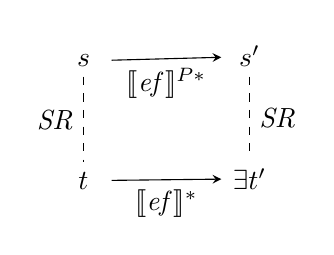
\begin{tikzpicture}
  \matrix (m) [matrix of math nodes,row sep=3em,column sep=4em,minimum width=2em]
  {
     s & s' \\
     t & \exists t' \\};
  \path[-stealth]
	(m-1-1) edge [dashed, -] node [left] {$\mathit{SR}$} (m-2-1)
			edge node [below] {$\llbracket \mathit{ef} \rrbracket^{P*}$} (m-1-2)
	(m-2-1) edge node [below] {$\llbracket \mathit{ef} \rrbracket^*$} (m-2-2)
	(m-1-2) edge [dashed, -] node [right] {$\mathit{SR}$} (m-2-2);
\end{tikzpicture}
	\end{figure}
\end{proof}

\section{Proof of theorem}

Similarly to lemmas, we separate the theorem into two parts, and alter it slightly to make it more consistent with what we have proved in Agda:

\begin{theorem}
\begin{multline*}
      \forall s, s', s'' \in \mathit{State^P} \ldotp\\\mathit{Init^P(s)} \land s \llbracket \mathit{(w \lor f)\ast} \cdot f \rrbracket^P s' \land s' \llbracket \mathit{w\ast} \cdot w^c \cdot \mathit{r^c\ast} \cdot r \rrbracket^P s'' \\ \implies \mathit{read(s')} \doteq \mathit{read(s'')}
\end{multline*}
\end{theorem}
\begin{proof}
	From $\mathit{initialisation}$ and repetively applying \cref{lemma-1} to the first relation, we have $\mathit{AR(s, t)}$ and $\mathit{AR(s', t')}$.
	The theorem can then be sketched as follows:
	\begin{figure} [h] \centering
		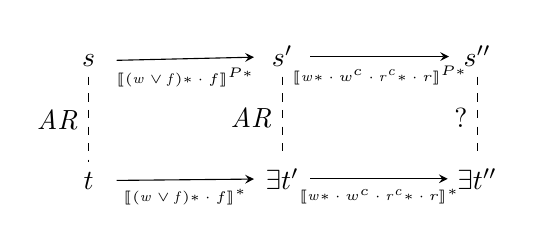
\begin{tikzpicture}
			\matrix (m) [matrix of math nodes, row sep=3em, column sep=5em, minimum width=2em]
			{ s & s' & s'' \\
			  t & \exists t' & \exists t'' \\};
			\path[-stealth]
			(m-1-1) edge [dashed, -] node [left] {$\mathit{AR}$} (m-2-1)
					edge node [below] {\tiny{$\llbracket \mathit{(w \lor f)*} \cdot f \rrbracket^{P*}$}} (m-1-2)
			(m-2-1) edge node [below] {\tiny{$\llbracket \mathit{(w \lor f)*} \cdot f \rrbracket^*$}} (m-2-2)
			(m-1-2) edge [dashed, -] node [left] {$\mathit{AR}$} (m-2-2)
					edge node [below] {\tiny{$\llbracket \mathit{w*} \cdot w^c \cdot \mathit{r^c*} \cdot r \rrbracket^{P*}$}} (m-1-3)
			(m-2-2) edge node [below] {\tiny{$\llbracket \mathit{w*} \cdot w^c \cdot \mathit{r^c*} \cdot r \rrbracket^*$}} (m-2-3)
			(m-1-3) edge [dashed, -] node [left] {?} (m-2-3);

		\end{tikzpicture}
	\end{figure}\\
	We can find some intermidiate states $s'_1$, $s'_2$, $s'_3$, and by applying \cref{lemma-1} repetively to obtain
	\begin{figure} [h] \centering
		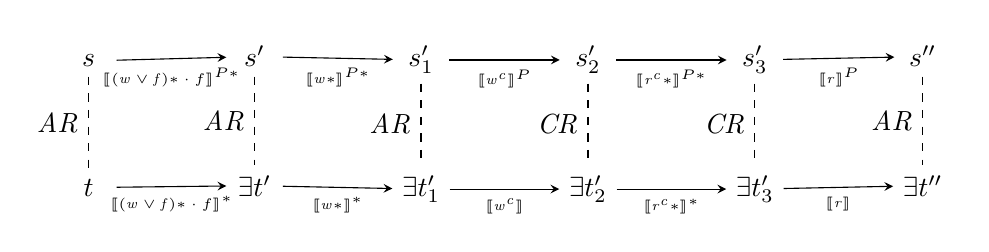
\begin{tikzpicture}
			\matrix (m) [matrix of math nodes, row sep=3em, column sep=4em, minimum width=2em]
			{ s & s' & s'_1 & s'_2 & s'_3 & s'' \\
			  t & \exists t' & \exists t'_1 & \exists t'_2 & \exists t'_3 & \exists t'' \\};
			\path[-stealth]
			(m-1-1) edge [dashed, -] node [left] {$\mathit{AR}$} (m-2-1)
					edge node [below] {\tiny{$\llbracket \mathit{(w \lor f)*} \cdot f \rrbracket^{P*}$}} (m-1-2)
			(m-2-1) edge node [below] {\tiny{$\llbracket \mathit{(w \lor f)*} \cdot f \rrbracket^*$}} (m-2-2)
			(m-1-2) edge [dashed, -] node [left] {$\mathit{AR}$} (m-2-2)
					edge node [below] {\tiny{$\llbracket \mathit{w*}  \rrbracket^{P*}$}} (m-1-3)
			(m-2-2) edge node [below] {\tiny{$\llbracket \mathit{w*} \rrbracket^*$}} (m-2-3)
			(m-1-3) edge [dashed, -] node [left] {$\mathit{AR}$} (m-2-3)
					edge node [below] {\tiny{$\llbracket \mathit{w^c}  \rrbracket^{P}$}} (m-1-4)
			(m-2-3) edge node [below] {\tiny{$\llbracket \mathit{w^c} \rrbracket$}} (m-2-4)
			(m-1-4) edge [dashed, -] node [left] {$\mathit{CR}$} (m-2-4)
					edge node [below] {\tiny{$\llbracket \mathit{r^c*}  \rrbracket^{P*}$}} (m-1-5)
			(m-2-4) edge node [below] {\tiny{$\llbracket \mathit{r^c*} \rrbracket^*$}} (m-2-5)
			(m-1-5) edge [dashed, -] node [left] {$\mathit{CR}$} (m-2-5)
					edge node [below] {\tiny{$\llbracket \mathit{r}  \rrbracket^{P}$}} (m-1-6)
			(m-2-5) edge node [below] {\tiny{$\llbracket \mathit{r} \rrbracket$}} (m-2-6)
			(m-1-6) edge [dashed, -] node [left] {$\mathit{AR}$} (m-2-6);

		\end{tikzpicture}
	\end{figure}\\
	thus complete the proof:
\begin{align*}
	\mathit{read(s)}   &\doteq \mathit{volatile(t)}   \tag{Observational Equivalence} \\
	& \qquad \quad \rotatebox{90}{$\doteq$} \tag{\cref{lemma-2-1}}\\
	\mathit{read(s'')} &\doteq \mathit{volatile(t'')} \tag{Observational Equivalence}
\end{align*} `
\end{proof}

\begin{theorem}
\begin{multline*}
      \forall s, s', s'', s''' \in \mathit{State^P} \ldotp\\\mathit{Init^P(s)} \land s \llbracket \mathit{(w \lor f)\ast} \cdot f \rrbracket^P s' \land
      s' \llbracket \mathit{w\ast} \rrbracket^P s'' \land
      s'' \llbracket f^c \cdot \mathit{r^c\ast} \cdot r \rrbracket^P s'''\\
      \implies \mathit{read(s')} \doteq \mathit{read(s''')} \lor \mathit{read(s'')} \doteq \mathit{read(s''')}
\end{multline*}
\end{theorem}


\end{document}
